%%%%%%%%%%%%%%%%%%%%%%%%%%%%%%%%%%%%%%%%%%%%%%%%%%%%%%%%%%%%%%%%%%%%%%%%%%%%%%%%
% TUM-Vorlage: Wissenschaftliche Arbeit
%%%%%%%%%%%%%%%%%%%%%%%%%%%%%%%%%%%%%%%%%%%%%%%%%%%%%%%%%%%%%%%%%%%%%%%%%%%%%%%%
%
% Rechteinhaber:
%     Technische Universität München
%     https://www.tum.de
% 
% Gestaltung:
%     ediundsepp Gestaltungsgesellschaft, München
%     http://www.ediundsepp.de
% 
% Technische Umsetzung:
%     eWorks GmbH, Frankfurt am Main
%     http://www.eworks.de
%
%%%%%%%%%%%%%%%%%%%%%%%%%%%%%%%%%%%%%%%%%%%%%%%%%%%%%%%%%%%%%%%%%%%%%%%%%%%%%%%%

%%%%%%%%%%%%%%%%%%%%%%%%%%%%%%%%%%%%%%%%%%%%%%%%%%%%%%%%%%%%%%%%%%%%%%%%%%%%%%%%
\input{./Ressourcen/Praeambel.tex} % !!! NICHT ENTFERNEN !!!
%%%%%%%%%%%%%%%%%%%%%%%%%%%%%%%%%%%%%%%%%%%%%%%%%%%%%%%%%%%%%%%%%%%%%%%%%%%%%%%%

\renewcommand{\Thema}{%
    MAIN-Seminar. Chap12. Matching Markets.}

%%%%%%%%%%%%%%%%%%%%%%%%%%%%%%%%%%%%%%%%%%%%%%%%%%%%%%%%%%%%%%%%%%%%%%%%%%%%%%%%
\input{./Ressourcen/Anfang.tex} % !!! NICHT ENTFERNEN !!!
%%%%%%%%%%%%%%%%%%%%%%%%%%%%%%%%%%%%%%%%%%%%%%%%%%%%%%%%%%%%%%%%%%%%%%%%%%%%%%%%
% \newcommand{\savefootnote}[2]{\footnote{\label{#1}#2}}
% \newcommand{\repeatfootnote}[1]{\textsuperscript{\ref{#1}}}

% \newtheorem{theorem}{Theorem}
\theoremstyle{definition}
\newtheorem{exmp}{Example}[section]
\declaretheorem{theorem} 
\declaretheoremstyle[%
  spaceabove=-6pt,%
  spacebelow=6pt,%
  headfont=\normalfont\itshape,%
  postheadspace=1em,%
  qed=\qedsymbol%
]{mystyle} 
\declaretheorem[name={Proof},style=mystyle,unnumbered,
]{prf}

\begin{document}

\title{Thema der Arbeit}
\author{Martin Mustermann}
\date{Datum}


% \tableofcontents % Inhaltsverzeichnis

% \chapter{Abstract}
% The Matching Markets Problem is a classic topic in computer science field as well as in the mathmatical field.
% This Handout proposes a introduction to the design of the matching market, which is stated as the Assigenment of the participant in some way. 
% The way they are assigned, called Matching, can depend on the type of Matching Markets, and the mind of the participants.
% First, the common convention for this Handout also for the Presentaion is introducted. Second, the Two-sided Matching is handled, which is a basic for the Marriage Problem as the third topic.
% Finally we will hanldle another type of matching - Assignment Problem. 

% Keywords: Two-sided Matching, Stability, Marriage Problem, Assigenment Problems

\chapter{Introduction to Matching}
% \section{Fundamental knowledge}
\section{Set and Strict Preference Order}
Before the real matching comes, it is the point to have the common conventions about our topic. There are some rules, which this handout and the presentaion are based on.
The participant is called \emph{agent}, and the set of all agnets is denoted by $X$, so each agent $x \in X$. A \emph{matching} $m$ in a set of machings $M$, so that $m \in M$, represents the output of a matching mechanism.
The \emph{strict preference order} is defined as preference, that a specific agent $x$ has on different matchings. 
% In addition, there are three types of preference order:
\vspace{-\baselineskip}
\begin{description}[leftmargin=1em+5mm, labelindent=5mm]
    % \item[Weak Preference]  Agent $x$ has a \textbf{weak preference order} $\succeq_x$, so that $m \succeq_x m'$, for matchings $m$ and $m'$, indicates that agent $x$ weakly prefers $m$ to $m'$.
    \item[Strict Preference - Definition]  Agent $x$ has a \emph{strict preference order} $\succ_x$, so that $m \succ_x m'$, for matchings $m$ and $m'$, indicates that agent $x$ strict prefers $m$ to $m'$. 
    % \item[] When $m \succeq_x m'$ and not $m' \succeq_x m$, then the agent has a \textbf{strict preference} for $m$ over $m'$, denoted $m \succ_x m'$. 
    % \item[Indifferent] It is allowed for $m \succeq_x m'$ and $m' \succeq_x m$, so that agent $x$ is \textbf{indifferent} between two machtings, written as $m \sim_x m'$.
\end{description}
\begin{exmp}
The man $x$ admiring the woman $y$ most in woman's set $Y$ can be formulated as: $\forall y' \in Y\setminus{y} : y \succ_x y'$ \\
% If the woman $y$ equally admires the man $x_1$ and the other man $x_2$. We can formulate that as: $x_1 \sim_y x_2$
\end{exmp}

\section{Three Types of Matching}
\vspace{5mm}
\vspace{-\baselineskip}
\begin{description}[leftmargin=1em+5mm, labelindent=5mm]    
    \item [Two-Sided Matching - Definition] is the matching, where there are two distinct groups of agents, and the problem is to match each agent on one side of the market with
    an agent on the other side. Stable Marriage Problem belongs to this type. 
    \item [Assignment Problems - Definition] is the matching, where there are items and agents with preferences on items, and  the problem is to assign a distinct item to each agent.
    \item [Kidney-Paired Donation - Definition] is the matching, where patient-donor pairs arrive to the market, and the problem is to determine how to match pairs such that the donor in one pair is compatible with
    the patient in another pair and vice versa, so that such a match enables two kidney transplants.
    \footnote{David C. Parkes, Sven Seuken. Economics and Computation. Chapter 12: Matching Markets(pp. 291-293). 2017}
\end{description} 
In this handout and the presentation we will only talk about the Two-Sided Matching and Stable Marriage Problem, which is a case based on the this type of matching.

\section{Matching in Graph}
\vspace{5mm}
\vspace{-\baselineskip}
\begin{description}[leftmargin=1em+5mm, labelindent=5mm] 
    \item [Unweighted Graphs - Definition] Let $G = (V,E)$ be any graph with $n$ vertices and $m$ edges. A matching $M$ of $G$ is a subset of $E$ such that no two edges in $M$ are adjacent. 
    We say that a vertex $v$ is matched in $M$ if there is other some vertices $M(v) \in V$ such that $\{v, M(v)\} \in M$. Otherwise, $v$ is unmatched in $M$.\footnote{David J. Abraham. Algorithmics of Two-Sided Matching Problems. 2003}
    \item [Bipartite graph - Definition] A graph $G = (V,E)$ is \emph{bipartite} if the vertex set  $V$ can be partitioned into two disjoint subsets such that for every edge $(u,v)\in E$,  $u$ and $v$ are in opposite subsets.\footnote{\url{https://en.wikibooks.org/wiki/Graph_Theory/Definitions}}
\end{description}

\subsection{Exercise}
Following are two graphs representing the matching between 2 sides. Which is a bipartite graph?
\begin{center}
    \begin{minipage}{.4\textwidth}
        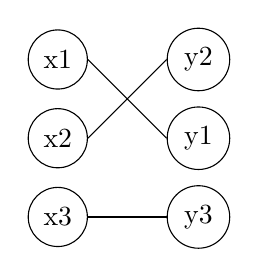
\begin{tikzpicture}
            \draw (0,2) node[anchor=east,circle, draw]{x1} -- (1,1) node[anchor=west, circle,draw]{y1};
            \draw (0,1) node[anchor=east,circle, draw]{x2} -- (1,2) node[anchor=west, circle,draw]{y2};
            \draw (0,0) node[anchor=east,circle, draw]{x3} -- (1,0) node[anchor=west, circle,draw]{y3};
        \end{tikzpicture} 
    \end{minipage}
    \begin{minipage}{.4\textwidth}
        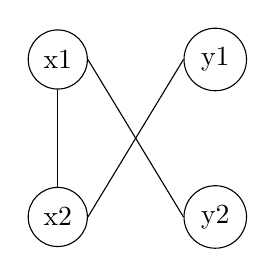
\begin{tikzpicture} 
            \node at (0,3) [circle, draw] (b1) {x1};
            \node at (0,1) [circle, draw] (b2) {x2};
            \node at (2,1) [circle, draw] (g1) {y2};
            \node at (2,3) [circle, draw] (g2) {y1};
            \draw (b1.east) -- (g1.west);
            \draw (b2.east) -- (g2.west);
            % \draw[red] (b1.south) -- (b2.north);
            \draw (b1.south) -- (b2.north);
        \end{tikzpicture}
    \end{minipage}
\end{center}


\chapter{Two-Sided Matching and Stable Marriage Problem}
% \section{Two-Sided Matching and Stable Marriage Problem}
\section{Description and Definition}
\begin{description}[leftmargin=1em+5mm, labelindent=5mm]
    \item[Two-side-matching Markets - Definiton]   \footnote{David C. Parkes, Sven Seuken. Economics and Computation. Chapter 12: Matching Markets(pp. 293 - 294). 2017} There are \textbf{two distinct groups of agents}. The problem is to match each agent in one group to an agent in the other group,
    such that no agent is matched to more than one other agent. This outcome is a matching.
    \item[Stable Marriage Problem - Description] The Stable Marriage Problem is a matching problem in graph theory first introduced
    by Gale and Shapley\footnote{D. Gale and L. S. Shapley. College admissions and the stability of marriage. The American Mathematical Monthly. 1962}. An instance of this problem consists of two sets, a set of men
    and a set of women. Each person specifies the order of all members of opposite sex. A
    matching is stable if there is no pair where both man and woman prefer each other
    to their current partner in the matching. The goal of this problem is to find a stable
    matching for a given instance. Gale and Shapley proved that there always exists such a
    matching for any instance. They also provided a polynomial algorithm for solving the
    problem. 
    \item[Stable Marriage Problem - Definition] An instance of the Stable Marriage Problem consists of a set of $n$
    men and a set of $n$ women where each man and each woman provides a lineary strict preference order 
    lists of all members of the opposite sex. Such lists are called preference lists.
    Let $M$ be an one-to-one correspondence between the subset of men and the subset
    of women, then $M$ is a marriage. If $(x, y) \in M$, called $(x, y)$
    as a pair in $M$, means $x$ is married with $y$ in $M$ and $y$ is married with $x$ in $M$.
    Furthermore, that a agent is unmatched in $M$ if he (or she) is not married
    with any woman (or man) in $M$, otherwise this agent is matched in $M$. Let $M(x)$
    denote the woman who is married with the man $x$ in $M$ and let $M(y)$ denote the man married
    with the woman $y$ in $M$. Agents have only the strict preferences in this problem.
    \footnote{Andrej Podhradsky. Stable Marriage Problem Algorithms. 2010}
\end{description}


\section{Prefer to be Unmatched}
An agent may prefer to be unmatched than matched with a particular agent on the other side.
\begin{exmp}
    Preference $\emptyset \succ_y $ shows the intention of a woman $y$ who strictly prefers not to be matched than to be matched with man $x$.
In this case, the man $x$ is said to be \emph{unacceptable} to the woman $y$. 
\end{exmp}

\section{Blocking Pair and Stable Marriage}
\begin{description}[leftmargin=1em+5mm, labelindent=5mm]
\item[Blocking Pair - Definition] Let $X$ be a set of men, $Y$ be a set of women, and $M$ be a marriage. A
pair $(x, y)$ is a blocking pair \footnote{Dan Gusfield, Robert W.Irving. The Stable Marriage Problem: Structure and Algorithms. Chapter 1: Elementary Concept and Result(pp. 6). The MIT Press, 1989} for $M$ if $(x, y) \notin M$ but:
\begin{itemize}[leftmargin=1em+8mm]
    \item $y$ prefers $x$ to $M(y)$ and
    \item $x$ prefers $y$ to $M(x)$
    \item If $\emptyset \succ_y M(y)$ for a woman $y$, then $(y, \emptyset)$ form a blocking pair. Similar for a man $x \in X$.
    % \item both $m$ and $w$ are free in $M$
    % \item $m$ is free in $M$ and $w$ prefers $m$ to $M(w)$
    % \item $w$ is free in $M$ and $m$ prefers $w$ to $M(m)$
\end{itemize}
\vspace{5mm}
\item[Unstable Marriage and Stable Marriage - Definition]If there is at least one blocking pair for $M$ then we say that $M$ a \emph{unstable marriage}, otherwise a \emph{stable marriage}.
A blocking pair also exists when an agent prefers to be unmatched rather than assigned to his/her match. \\
\end{description}
% \hspace{5mm}
\textbf{Yes-No Questions}: Are the following statements true?
\begin{itemize}[leftmargin=1em+8mm]
    % \item Men $x$ and woman $y$ form a blocking pair $(x, y)$ for matching $M$ if $M(x) \neq y$ and $M(x) \neq y$.
    \item A stable matching is one in which no pair of agents prefer each other over their respective matches.
    \item If $x$ is unmatched in $M$ and $y$ prefers $x$ to $M(y)$ means that: $x \succ_y M(y)$ 
    % ($x$ is better than the match of $y$).
    % \item If $\emptyset \succ_x M(x)$ for a men $x$, then $(x, \emptyset)$ form a blocking pair. 
\end{itemize}
% A stable matching is one in which no pair of agents prefer each other over their respective matches.
% A matching $\mu$ is stable if and only if there is no blocking pair.
% This requires there to be no pair of agents who prefer each other to their assigned matches, i.e., no blocking pair.
% A blocking pair also exists when an agent prefers to be unmatched rather than assigned to her match. The concern is that if there was such a pair of agents then the outcome would be unstable, and they might break away and do something that they both prefer. Stability also requires that there is no agent who prefers to be unmatched than receive her assigned match.
\subsection{Exercise} 
Suppose that there are three men and three women, with strict preference orders: \\  
\centerline{$y_2 \succ_{x_1} y_1 \succ_{x_1} y_3$}  \\
\centerline{$y_1 \succ_{x_2} y_3 \succ_{x_2} y_2$}  \\
\centerline{$y_1 \succ_{x_3} y_2 \succ_{x_3} y_3$}  \\
\centerline{$x_1 \succ_{y_1} x_3 \succ_{y_1} x_2$} \\  
\centerline{$x_3 \succ_{y_2} x_1 \succ_{y_2} x_2$} \\ 
\centerline{$x_1 \succ_{y_3} x_3 \succ_{y_3} x_2$} \\
% \vspace{3mm}
% Can you re-write these orders in a set notation? \\
Can you judge the following graphs, if they are stable?

\begin{center}
    \begin{minipage}{.3\textwidth}
        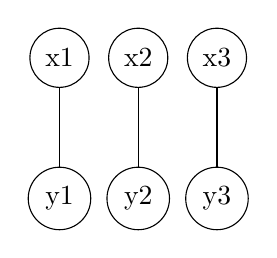
\begin{tikzpicture}
            \draw (0,0) node[anchor=north,circle, draw]{y1} -- (0,1) node[anchor=south, circle,draw]{x1};
            \draw (1,0) node[anchor=north,circle, draw]{y2} -- (1,1) node[anchor=south, circle,draw]{x2};
            \draw (2,0) node[anchor=north,circle, draw]{y3} -- (2,1) node[anchor=south, circle,draw]{x3};
        \end{tikzpicture}
    \end{minipage}
    \begin{minipage}{.3\textwidth}
        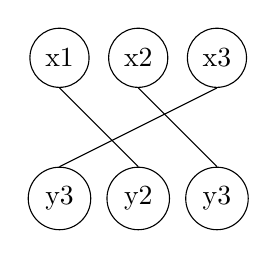
\begin{tikzpicture}
            \draw (1,0) node[anchor=north,circle, draw]{y2} -- (0,1) node[anchor=south, circle,draw]{x1};
            \draw (2,0) node[anchor=north,circle, draw]{y3} -- (1,1) node[anchor=south, circle,draw]{x2};
            \draw (0,0) node[anchor=north,circle, draw]{y3} -- (2,1) node[anchor=south, circle,draw]{x3};
        \end{tikzpicture}
    \end{minipage}
\end{center}

\clearpage
\section{Gale–Shapley Deferred Acceptance Algorithm}
    The following is an algorithm by Dale Gale and Lloyd Shapley \footnote{D. Gale and L. S. Shapley. College admissions and the stability of marriage. The American Mathematical Monthly (pp.69:9–15). 1962} in 1962 to find such a stable matching. The algorithm is like actual human behavior.
    This algorithm takes a list preference order as its input and output of it is a stable marriage. With the help of that, a \textbf{stable marriage} could be found.
    Deferred Acceptance Algorithm has agents on one side make offers to agents on the other side. The agent on the other side will tentaively agree on acceptable offers unless a better offer comes along. 
    There are two versions of Deferred Acceptance Algorithm, depending on which side makes the offers.	In the running example about marriage problem, we refer to these versions as the men-proposing algorithm and the woman-proposing algorithm.   
	We describe the men-proposing version in the Algorithm 1 below. The woman-proposing version is defined analogously. Noted that if the two versions of Deferred Acceptance Algorithm return different matching, there may be more than one stable matching.
    \\ 

    \begin{algorithm}[H]
        \SetKwInOut{Input}{Input}
        \SetKwInOut{Output}{Output}
    
        % \underline{function Euclid} $(a,b)$\;
        \Input{a list of preference order}
        \Output{a stable marriage $M$}
        \underline{Initialize} $M$ to empty matching.\\
        \While{Some man $x$ is unmatched and hasn't proposed to every woman}
          {
            $x$ proposes to the most preferred woman $y$ to whom he has not yet propose\;
            \uIf{$y$ is unmatched}
            {
                add $(x, y)$ to the Matching $M$\; 
            }
            \uElseIf{$y$ prefers $x$ to current partner $x'$}
            {
                Replace $(x', y)$ with $(x, y)$ in Matching $M$\;
            }
            \Else
            {
                $y$ rejects $x$\;
            }
          }
        \caption{Gale–Shapley Deferred Acceptance Algorithm (men-proposing version) \footnote{See footnote 5 below}}
    \end{algorithm}
 
	% \subsection{Boy-proposing DA mechanism}
	% Each girl starts off being matched with $\emptyset$. DA proceeds in rounds:  
	% \begin{itemize}
	% 	\item (round $1$) Each boy proposes to her top-ranke  girl (perhaps $\emptyset$). Each girl tentatively accepts the top-ranked proposal she receives (holding onto $\phi$ if this is preferred) and
	%  rejects the other proposal .
	%   \item (round $k$, $k > 1$). Each boy whose most recent proposal was rejected proposes to her top-ranked girl who has not yet rejected her proposal, or $\phi$ if this is now top-ranked amongst
	% 	the remaining options.  
	% 	\item  The mechanism terminates when no new proposals are made. At this point, each boy is matched with the girl (perhaps $\phi$) to whom she made her final proposal, and each girl is matched with the proposal she holds (perhaps $\phi$).
	% \end{itemize} 

\subsection{Exercise}
Try to apply \textbf{Gale–Shapley Deferred Acceptance Algorithm} on Exercise $2.3.1$. Write down every step that you need.
% \vspace{1cm}
% \begin{theorem}
%     Everybody gets married.
% \end{theorem}
% \begin{prf}
%     First note that once a man is proposed to, he is engaged to be married
%     and will never lose that. He can only trade up to better woman for matching on his list. And
%     since each woman was ranked by every man, the only way that a woman will not be
%     married is if she is rejected by every man. 
%     Assume there exists a woman that is not married, then there also must be man who is unmarried. But this unmarried
%     man must have been proposed to at one point by the unmarried woman, thus he
%     must be married. Contradiction, so everybody gets married.
% \end{prf}

% \begin{theorem}
%     The Gale–Shapley deferred acceptance algorithm produces a stable matching.
% \end{theorem}   
% \begin{prf}
%     Assume the opposite, that the matching is not stable. So there must be at least one
% blocking pair, $(x, y)$. Suppose $x$ married $y'$ (who he likes less than $y$) and that
% $y$ married $x'$ (who she likes less than $x$). That means $x$ must have proposed to
% $y$ at one point and she rejected him. But the only way that $y$ would reject $x$ is if
% she had a proposal from somebody she liked better. But women can only trade up
% from round to round, which means she must like $x'$ better than $y$. Contradiction,
% so the matching must be stable.
% \end{prf}

% \begin{theorem}
%     The algorithm terminates in at most $N * (N - 1) + 1$ rounds
% \end{theorem}   
% \begin{prf}
%     This just puts an upper-bound on the number of rounds that can take place
%     in this algorithm. Notice that at every round except the last round, a man crosses
%     a woman off his list. And since every man gets married, he can cross off no more
%     than $(N - 1)$ women. So there are no more than $N * (N - 1)$ cross-offs and thus no
%     more than $N*(N - 1) + 1$ rounds.
% \end{prf}




























% \chapter{}


% \begin{figure}[!ht]
% \noindent\hspace{0.5mm}\includegraphics[width=12cm]{./Ressourcen/Desert.jpg}
% \caption{Titel, Autor}
% \end{figure}

% \clearpage 

% Passen Sie gegebe  nenfalls die Ränder an die Vorgaben Ihres Prüfers an und
% beachten Sie dabei, dass das Logo der TUM sich oben rechts innerhalb der
% Ränder, auf der Titelseite befindet. Für die Titelseiten stehen separate
% Vorlagen zur Verfügung.

% Zur Definition von \gls{abk} erstellen Sie für die gewünschte Abkürzung einen
% Eintrag in der Datei \texttt{Abkuerzungen.tex} und referenzieren sie ihn
% mittels \texttt{\textbackslash{}gls}; diese tauchen nach einem Lauf mit
% \texttt{latexmk} im Abkürzungsverzeichnis auf. Beispiel:

% \vspace{-\baselineskip}
% \begin{description}[leftmargin=1em+5mm, labelindent=5mm]
% \item[Definition in \texttt{Abkuerzungen.tex}:] \texttt{\textbackslash{}newacronym\{abk\}\{Abk.\}\{Abkürzungen\}\}}
% \item[Referenzierung:] \texttt{\textbackslash{}gls\{abk\}}
% \end{description}

% Für weitere Informationen zu Glossaren und Abkürzungen siehe die Dokumentation
% des Pakets \texttt{glossaries} und die entsprechenden Abschnitte in den
% Vorlagendateien.


% \subsection[]{Aufzählungen}

% \begin{itemize}
% \item Dies ist die Standardaufzählung
%     \begin{itemize}
%     \item Dies ist die nächste Ebene der Aufzählung
%     \end{itemize}
% \end{itemize}


% \subsection[]{Nummerierungen}

% \begin{enumerate}
% \item Erster Punkt der Nummerierungen
%     \begin{enumerate}
%     \item Unterpunkt der Nummerierungen
%     \end{enumerate}
% \end{enumerate}
% \clearpage

% \listoffigures % Abbildungsverzeichnis

% \printacronyms[title={Abkürzungsverzeichnis}] % Abkürzungsverzeichnis

% \listoftables % Tabellenverzeichnis

% \onehalfspacing

% \addchap{Tabellenvarianten}

% \vspace{22mm}
% \section*{Überschrift Tabelle 1}

% \begin{table}[!h]
% \begin{tabularx}{\textwidth + 5pt}{@{\hspace{3pt}} M | @{\hspace{3pt}} M}
% \multicolumn{2}{@{}X}{%
%     \begin{tabularx}{\textwidth}{@{\hspace{3pt}} M @{\hspace{14.5pt}} M}
%     \textbf{Spalte 1} & \textbf{Spalte 2}
%     \end{tabularx}%
% } \\
% \hline
% Nummer 1 & Nummer 2 \\
% \hline
% Nummer 1 & Nummer 2 \\
% \hline
% Nummer 1 & Nummer 2 \\
% \hline
% \end{tabularx}

% \caption{Beschreibung}
% \end{table}


% \vspace{\parskip}
% \section*{Überschrift Tabelle 2}

% \begin{table}[!h]
% \hspace{-5pt}
% \begin{tabularx}{\textwidth + 5pt}{| @{\hspace{3pt}} M | @{\hspace{3pt}} M |}
% \hline
% \textbf{Spalte 1} & \textbf{Spalte 2} \\
% \hline
% Nummer 1 & Nummer 2 \\
% \hline
% Nummer 1 & Nummer 2 \\
% \hline
% Nummer 1 & Nummer 2 \\
% \hline
% \end{tabularx}
% \caption{}
% \end{table}


% \vspace{\parskip}
% \section*{Überschrift Tabelle 3}

% \begin{table}[!h]
% \begin{tabularx}{\textwidth}{@{} M M}
% \textbf{Spalte 1} & \textbf{Spalte 2} \\
% Nummer 1 & Nummer 2 \\
% Nummer 1 & Nummer 2 \\
% Nummer 1 & Nummer 2 \\
% \end{tabularx}
% \caption{}
% \end{table}

% \clearpage

% \addchap{Tabellenvarianten 2}

% \vspace{22mm}
% \section*{Überschrift Tabelle 1}

% \begin{table}[!h]
% \fontsize{9pt}{13pt}\selectfont
% %\renewcommand{\arraystretch}{1.8}
% \hspace{-5pt}
% \begin{tabularx}{\textwidth + 5pt}{@{\hspace{3pt}} M | @{\hspace{3pt}} M}
% \multicolumn{2}{@{}X}{%
%     \begin{tabularx}{\textwidth}{@{\hspace{3pt}} M @{\hspace{14.5pt}} M}
%     \textbf{Spalte 1} & \textbf{Spalte 2}
%     \end{tabularx}%
% } \\
% \hline
% Nummer 1,\newline\,mehrzeilig in Schriftgröße 9 pt & Nummer 2 \\
% \hline
% Nummer 1 & Nummer 2 \\
% \hline
% Nummer 1 & Nummer 2 \\
% \hline
% \end{tabularx}

% \caption{}
% \end{table}


% \vspace{\parskip}
% \section*{Überschrift Tabelle 2}

% \begin{table}[!h]
% \fontsize{9pt}{13pt}\selectfont
% \hspace{-5pt}
% %\renewcommand{\arraystretch}{1.8}
% \begin{tabularx}{\textwidth + 5pt}{| @{\hspace{3pt}} M | @{\hspace{3pt}} M |}
% \hline
% \textbf{Spalte 1} & \textbf{Spalte 2} \\
% \hline
% Nummer 1 & Nummer 2 \\
% \hline
% Nummer 1 & Nummer 2 \\
% \hline
% Nummer 1 & Nummer 2 \\
% \hline
% \end{tabularx}
% \caption{}
% \end{table}


% \vspace{\parskip}
% \section*{Überschrift Tabelle 3}

% \begin{table}[!h]
% \fontsize{9pt}{13pt}\selectfont
% %\renewcommand{\arraystretch}{1.8}
% \begin{tabularx}{\textwidth}{@{} M M}
% \textbf{Spalte 1} & \textbf{Spalte 2} \\
% Nummer 1 & Nummer 2 \\
% Nummer 1 & Nummer 2 \\
% Nummer 1 & Nummer 2 \\
% \end{tabularx}
% \caption{}
% \end{table}

\end{document}